\chapter{Фотоны. Фотоэффект. Закон Эйнштейна. Опыт Боте. Тормозное 
рентгеновское излучение. Эффект Комптона. Давления света.}

Фотоны - это кванты света. Фотоны не имеют массы покоя и электрического заряда.
Спин фотона равен 1.

Согласно закону пропорциональности массы и энергии и гипотезе Планка, энергия
фотона определяется формулой: \( E = \hbar\omega = h\nu \). Фотон -- частица, не
обладающая массой покоя. Она может существовать, только двигаясь со скоростью
света \( c \). Инертная масса фотона: \( m = E/c^2 = h\nu/c^2 \).

Найдем связь энергии с импульсом фотона.

Релятивистское выражение для импульса: \( \ds p = \frac{m_0v}{\sqrt{1 -
\frac{v^2}{c^2}}} \).

Для энергии: \( \ds E = \frac{m_0c^2}{\sqrt{1 - \frac{v^2}{c^2}}} \).

Выразим из первого выражения квадрат скорости \( \ds v^2 = \frac{p^2c^2}{p^2 +
m_0^2c^2} \) и подставим его во второе:
\[
    E = \frac{m_0c^2}{\sqrt{1 - \frac{p^2c^2}{(p^2 + m_0^2c^2)c^2}}} =
    \frac{m_0^2c^2}{\sqrt{\frac{p^2 + m_0^2p^2 - p^2}{p^2 + m_0^2c^2}}} =
    c\sqrt{p^2 + m_0^2c^2} = pc.
\]
Таким образом, импульс фотона: \( p = h\nu/c = \hbar\omega/c = \hbar k =
h/\lambda \). Через волновой вектор импульс выражается следующим образом:
\( \vec{p} = \hbar\vec{k} \).

Идея Планка нашла своё подтверждение при объяснении явления фотоэффекта.

Фотоэффект бывает трёх видов:
\begin{enumerate}
    \item внешний -- явление испускания веществом электронов под действием
    внешнего электромагнитного излучения;
    \item внутренний -- вызванные электромагнитным излучением переходы
    электронов внутри полупроводника или диэлектрика из связанных состояний в
    свободные без вылета наружу;
    \item вентильный -- это возникновение ЭДС при освещении контакта двух разных
    полупроводников или полупроводника и металла (при отсутствии внешнего
    электрического поля).
\end{enumerate}

\begin{figure}[h!]
    \center
    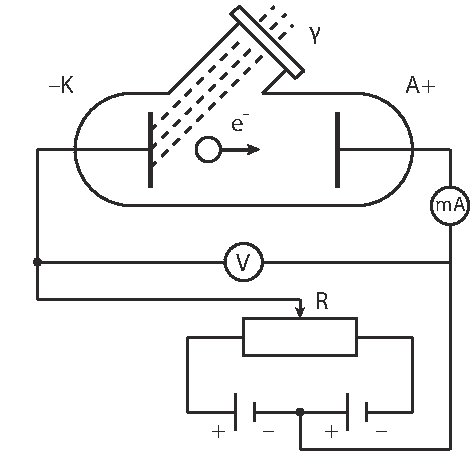
\includegraphics[width=.32\textwidth]{02_01}
    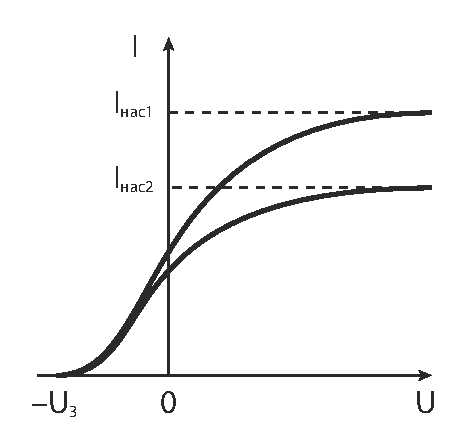
\includegraphics[width=.32\textwidth]{02_02}
    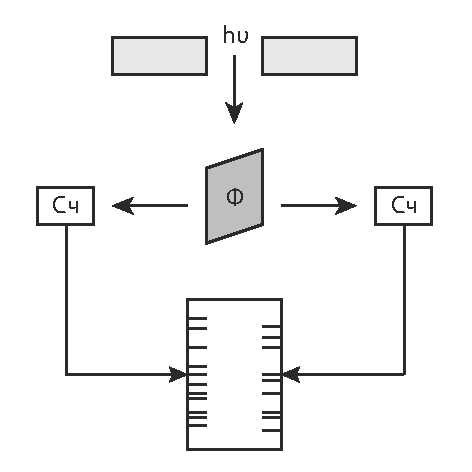
\includegraphics[width=.32\textwidth]{02_03}
    \parbox{.32\textwidth}{\caption{Принципиальная схема установки}
    \label{pic2_1}}
    \parbox{.32\textwidth}{\caption{ВАХ фототока}\label{pic2_2}}
    \parbox{.32\textwidth}{\caption{Схема опыта Боте}\label{pic2_3}}
\end{figure}
Первые фундаментальные исследования фотоэффекта выполнены русским ученым
А.~Г.~Столетовым. Принципиальная схема для исследования фотоэффекта приведена на
рис. \ref{pic2_1}: два электрода (катод \( K \) из исследуемого материала и
анод \( A \), в качестве которого Столетов применял металлическую сетку) в
вакуумной трубке подключены к батарее так, что с помощью потенциометра \( R \)
можно изменять не только значение, но и знак подаваемого на них напряжения. Ток,
возникающий при освещении катода монохроматическим светом (через кварцевое
стекло), измеряется включенным в цепь миллиамперметром.

Вольт-амперная характеристика фотоэффекта -- зависимость фототока \( I \),
образуемого потоком электронов, от напряжения (рис. \ref{pic2_2}).

Такая зависимость соответствует двум различным энергетическим освещенностям
катода (частота света в обоих случаях одинакова). По мере увеличения \( U \)
фототок постепенно возрастает, то есть все большее число фотоэлектронов
достигает анода. Пологий характер кривых показывает, что электроны вылетают из
катода с различными скоростями. Максимальное значение фототока насыщения
\( I_\emph{нас} \) определяется таким значением напряжения \( U \), при котором
все электроны, испускаемые катодом, достигают анода: \( I_\emph{нас} = ne \),
где \( n \) – число электронов, испускаемых катодом в 1 с.

Из ВАХ следует, при отсутствии подаваемого напряжения \( U \) фототок не
исчезает. Следовательно, электроны, выбитые из катода, обладают некоторой
начальной скоростью \( v \), а значит и отличной от нуля кинетической энергией,
поэтому они могут достигнуть катода без внешнего поля. Для того, чтобы фототок
стал равным нулю, необходимо приложить задерживающее напряжение
\( U_\emph{з} \). В этом случае ни один из электронов, даже обладающий при
вылете из катода максимальной скоростью \( v_{max} \), не может преодолеть
задерживающего поля и достигнуть анода. Следовательно,
\[
    \frac{mv_{max}^2}{2} = eU_\emph{з},
\]
то есть замерив задерживающее напряжение, можно определить максимальные значения
скорости и кинетической энергии фотоэлектрона.

А.Г. Столетов установил три закона фотоэффекта:
\begin{enumerate}
    \item при фиксированной частоте падающего света число фотоэлектронов,
    вырываемых из катода в единицу времени, пропорционально интенсивности света
    (сила тока насыщения пропорциональна энергетической освещенности \( E_e \)
    катода);
    
    \item максимальная начальная скорость фотоэлектронов не зависит от
    интенсивности падающего света, а определяется только его частотой \( \nu \);
    
    \item для каждого вещества существует красная граница фотоэффекта, то есть
    минимальная частота света, ниже которой фотоэффект невозможен.
\end{enumerate}

Эйнштейн развил гипотезу Планка для объяснения явления фотоэффекта: свет не
только испускает, но и распространяется и поглощается в виде отдельных квантов
энергии, получивших название фотоны: \( E_\emph{ф} = W_\emph{к} + A_\emph{вых}
\).
Работа выхода \( A_\emph{вых} \) существенным образом зависит от двух факторов:
\begin{enumerate}
    \item состояние поверхности металла;
    \item расстояние до поверхности.
\end{enumerate}

Формула Эйнштейна для внешнего фотоэффекта: \( \ds \hbar\omega = A_\emph{вых} +
\frac{mv_{max}^2}{2} \). Она непосредственно объясняет 2 и 3 закон Столетова. 
Красная граница фотоэффекта определяется следующим образом: \( \omega_\emph{кр}
= A_\emph{вых}/\hbar \).

\section{Опыт Боте}
Наиболее непосредственное подтверждение гипотезы Эйнштейна дал опыт Боте, в
котором использовался метод совпадения (рис. \ref{pic2_3}).

Тонкая металлическая фольга \emph{Ф} помещалась между двумя газоразрядными
счетчиками \emph{Сч}. Фольга освещалась слабым пучком рентгеновских лучей, под
действием которых она сама становилась источником рентгеновских лучей (это
явление называется рентгеновской флуоресценцией). Вследствие малой интенсивности
первичного пучка, количество квантов, испускаемых фольгой, было невелико. При
попадании квантов на счетчик механизм срабатывал и на движущейся бумажной ленте
делалась отметка. Если бы излучаемая энергия распространялась равномерно во все
стороны, как это следует из волновых представлений, оба счетчика должны были
срабатывать одновременно и отметки на ленте приходились бы одна против другой. В
действительности же наблюдалось совершенно беспорядочное расположение отметок.
Это можно объяснить лишь тем, что в отдельных актах испускания возникают
световые частицы, летящие то в одном, то в другом направлении. Так было
экспериментально доказано существование фотонов.

\begin{figure}[h!]
    \center
    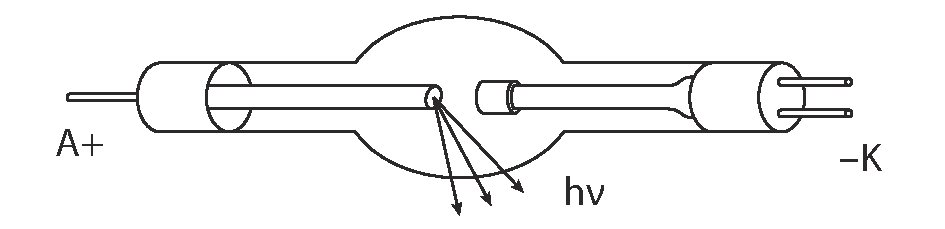
\includegraphics[width=.64\textwidth]{02_04} \hfill
    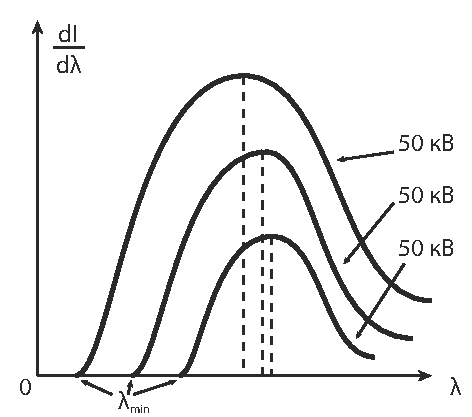
\includegraphics[width=.32\textwidth]{02_05}
    \parbox{.64\textwidth}{\caption{Схема установки для наблюдения тормозного
    рентгеновского излучения}\label{pic2_4}} \hfill
    \parbox{.32\textwidth}{\caption{Коротковолновая граница рентгеновского
    спектра}\label{pic2_5}}
\end{figure}

\section{Тормозное рентгеновское излучение}
Квантовая природа излучения подтверждается также существованием коротковолновой
границы тормозного рентгеновского спектра.

Тормозное рентгеновское излучение возникает при торможении пучка в быстро
движущихся электронов в веществе. За счёт термоэлектронной эмиссии из катода
вылетают электроны ускоренные внешнем полем и попадают на анод. В результате
торможения внутри анода испускаются электромагнитные волны, максимальная
интенсивность которых находится в рентгеновской области (рис. \ref{pic2_4}).

Начальная скорость электрона при попадании на анод определяется по формуле:
\[
    v_0 = \sqrt{\frac{2eU}{m}}, \text{ где } U \text{ -- ускоряющее напряжение}.
\]

Согласно классической электродинамике при торможении электрона должны возникать
излучения всех длин волн от нуля до бесконечности. Длина волны, на которую
приходится максимум мощности излучения, должна уменьшиться по мере увеличения
скорости электронов, что в основном подтверждается на опыте (рис. \ref{pic2_5}).
Однако есть принципиальное отличие от классической теории: нулевые распределения
мощности не идут к началу координат, а обрываются при конечных значениях
\( \lambda_{min} \) -- это и есть коротковолновая граница рентгеновского
спектра.

Существование коротковолновой границы непосредственно вытекает из квантовой
природы излучения. Действительно, если излучение возникает за счёт энергии,
теряемой электроном при торможении, то энергия кванта \( h\nu \) не может
превысить энергию электрона \( eU \), то есть \( h\nu \le eU \), отсюда
\( \nu = eU/h \) или \( \lambda_{min} = c/\nu_{min} = ch/eU \).

\begin{figure}[h!]
    \center
    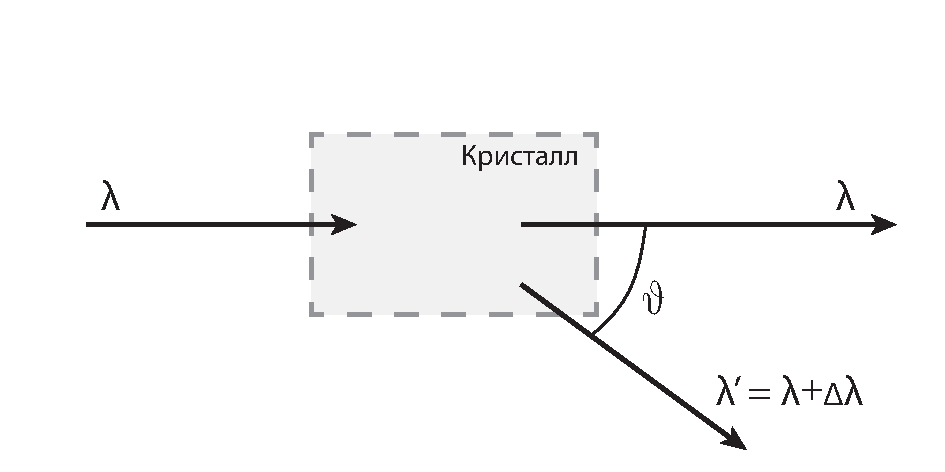
\includegraphics[width=.58\textwidth]{02_lec} \hfill
    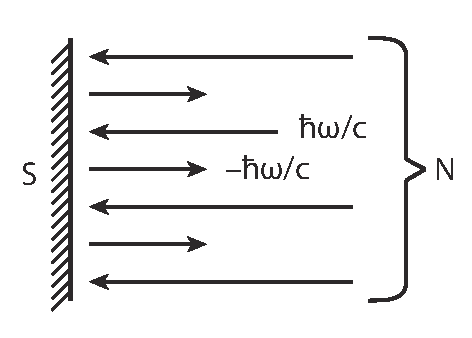
\includegraphics[width=.35\textwidth]{02_06}
    \parbox{.58\textwidth}{\caption{Эффект Комптона}\label{pic2_lec}} \hfill
    \parbox{.35\textwidth}{\caption{Давление света}\label{pic2_6}}
\end{figure}

\section{Эффект Комптона}
Упругое рассеяние коротковолнового электромагнитного излучения на свободных или
слабо связанных электронов (рис. \ref{pic2_lec}).

Было обнаружено, что в составе рассеянного излучения наряду с излучениями
первоначальные длины волны наблюдается также более длинноволновое излучение,
причем \( \Delta\lambda \) независимо от природы рассеиваемого вещества, не
зависит от длины волны падающего излучения, а зависит только от угла
рассеяния \( \theta \):
\[
    \Delta\lambda = \frac{2\pi\hbar}{m_ec}(1 - \cos\theta) = \Lambda(1 -
    \cos\theta).
\]

\section{Давление света}
Рассмотрим монохроматический пучок, который подает перпендикулярно на мишень с
коэффициентом отражения \( \rho \). Пусть \( N \) -- число фотонов падающих на
единицу поверхности мишени в единицу времени. Тогда от этой мишени отразится
\( \rho N - N_\emph{отраж}/(S\cdot\Delta t) \), а поглотится, соответственно,
\( (1 - \rho)N - N_\emph{погл}/(S\cdot\Delta t) \) (рис. \ref{pic2_6}). Мишени
передастся импульс \( \Delta p = p_0 - (-p_0) = 2p_0 = 2\hbar\omega/c \).

Тогда давление:
\[
    P = \frac{F}{S} = \frac{\Delta p}{S\Delta t} = \rho N\frac{2\hbar\omega}{c}
    + (1 - \rho)N\frac{\hbar\omega}{c} = (1 + \rho)N\frac{\hbar\omega}{c} =
    (1 + \rho)\frac{j}{c} = (1 + \rho)u,
\]
где \( j = N\hbar\omega \) -- плотность потока энергии, \( u = jc \) --
плотность энергии.

\newpage
